\documentclass[a4paper, 10pt, final]{article}
\usepackage{bonde}

\def\mytitle{Signal and Image Processing 2010}
\def\mysubtitle{Handin of mandatory excercise 7}
\def\myauthor{Ulrik Bonde}
\def\mymail{\mailto{bonde@diku.dk}}
\def\mydate{\today}
\def\repository{\url{http://github.com/bonde/sip}}

\title{\mytitle}
\subtitle{\mysubtitle}

\author{\myauthor{} - \mymail}
\date{\mydate}

\hypersetup{
colorlinks,%
citecolor=black,%
filecolor=black,%
linkcolor=black,%
urlcolor=black,%
bookmarksopen=false,
pdftitle={\mytitle{} - \mysubtitle},
pdfauthor={\myauthor}
}

\begin{document}
\maketitle

\subsection*{Question 7.1}
In this assignment we should implement the Hough transform using two
different approaches. The final goal is to detect lines in the image
shown in fig. \ref{apple}.

\begin{figure}[h!]
    \centering
    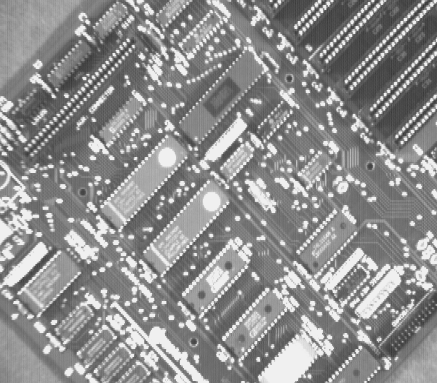
\includegraphics[angle=0,width=0.7\textwidth]{images/apple}
    \caption{Original image. Note that the image has a fair amount of
    noise, mostly periodic, vertical lines.}
    \label{apple}
\end{figure}

Only the actual Hough transform have been implemented. To find the
actual lines from the output of the Hough transform, the built-in
methods from the MATLAB image library called \texttt{houghpeaks} and
\texttt{houghlines} are used. Also, the Hough transform take an
edge-detected image as input. For this the Canny edge detection from
MATLAB is used.

Finally the implementations calculate the structure tensor as the
supplied code from Jon Sporring and also use his method \texttt{scale}
for scaling and determining derivatives.

\paragraph{1)}
The first implementation is only just mentioned in \citep[section
16.5.2, p. 458-460]{jahne-digital}. We use that a line can be
represented as
\begin{equation}
    x\cos\theta+y\sin\theta = \rho
\end{equation}
Now lines in the image can be represented in the parameter space by
their values of $\theta$ and $\rho$. We construct a $\rho\times\theta$
image which is called the Hough accumulator.

Now, we need to know the maximum value for $\rho$ when we want to
allocate an image for the accumulator. This is found by
\begin{equation}
    D = \sqrt{(M - 1)^2 + (N - 1)^2}
\end{equation}

For each point of interest we then calculate $\rho$ using values of
$\theta$ ranging from -90 to 90 with a variable step size for precision
at a computational cost. For each computation of $\rho$ we then
increase the accumulator at the position $(\rho, \theta)$.

\paragraph{2)}

%%%%%%%%%%%%%%%%%%%%%%%%%%%%%%%%%%%%%%%%%%%%%%%%%%%%%%%%%%%%%%%%%%%%
% Formal stuff

\bibliographystyle{abbrvnat}
\bibliography{bibliography}
%\addcontentsline{toc}{chapter}{Litteratur}

\appendix
\lstset{language=Matlab, basicstyle=\scriptsize,
    showstringspaces=false, numbers=left, stepnumber=1,
    numberstyle=\tiny, frame=none}
\section{Source code}
The full source can be viewed and downloaded from my repository at
\repository{}.

\subsection{SIPHoughTransform.m}
\lstinputlisting{../src/SIPHoughTransform.m}

\subsection{SIPFastHoughTransform.m}
\lstinputlisting{../src/SIPFastHoughTransform.m}

\end{document}

% vim: set tw=72 spell spelllang=en:
